% This is samplepaper.tex, a sample chapter demonstrating the
% LLNCS macro package for Springer Computer Science proceedings;
% Version 2.21 of 2022/01/12
%
\documentclass[runningheads]{llncs}

\usepackage{hyperref}
%
\usepackage[T1]{fontenc}
% T1 fonts will be used to generate the final print and online PDFs,
% so please use T1 fonts in your manuscript whenever possible.
% Other font encondings may result in incorrect characters.
%
\usepackage{graphicx}
% Used for displaying a sample figure. If possible, figure files should
% be included in EPS format.
%
% If you use the hyperref package, please uncomment the following two lines
% to display URLs in blue roman font according to Springer's eBook style:
\usepackage{color}
\renewcommand\UrlFont{\color{blue}\rmfamily}
\usepackage{amsmath} 
\usepackage{multirow} 
%
\begin{document}
%
\title{Analysis and elimination of bottlenecks in parallel algorithm for solving global optimization problems}
%
\titlerunning{Analysis and elimination of bottlenecks in parallel algorithm}
% If the paper title is too long for the running head, you can set
% an abbreviated paper title here
%
\author{
Konstantin Barkalov \orcidID{0000-0001-5273-2471} \and
Ilya Lebedev \orcidID{0000-0002-8736-0652} \and
Denis Karchkov \orcidID{0000-0002-4164-5927}
}
%
\authorrunning{K. Barkalov, I. Lebedev, D. Karchkov}
% First names are abbreviated in the running head.
% If there are more than two authors, 'et al.' is used.
%
\institute{Lobachevsky State University of Nizhny Novgorod, Nizhny Novgorod, Russia \\
\email{\{konstantin.barkalov,ilya.lebedev,karchkov\}@itmm.unn.ru}
}

%
\maketitle              % typeset the header of the contribution
%
\begin{abstract}
The paper presents the results of investigation of efficiency of the parallelization of a global optimum search algorithm. Two stages of solving the problem were distinguished: the search of a rough approximation to the global solution and its local refining. The novelty of the parallel algorithm considered in the present pa-per consists in the parallelization of the whole computational process -- both at the global search stage and at the one of the local refining of the solution found. The theoretical estimates of the algorithm parallelization efficiency are presented. The computational experiments were carried out. The results of the ones confirmed the theoretical conclusions.

\keywords{First keyword  \and Second keyword \and Another keyword.}
\end{abstract}
%
%
%
\section{Introduction}

The paper is devoted to the investigation of the parallel algorithms for solving complex optimization problems arising in various fields of science and technology. Several examples of such problems are presented in the review \cite{Pinter2006}.

As a rule, the objective function $\varphi(y)$ in such problems is a ``black-box'' function, i.e. it is defined not by a formula but as a software-implemented algorithm for computing its values at the points of the search domain $D$. In this case, the analytical methods for the search of the exact problem solution $y^{*}  \in D$ are not applicable, and its numerical solving is reduced to the construction of an approximate solution $y_k^* \in D, \|y^{*} - y_k^*\| \leq \varepsilon$, where $\varepsilon > 0$ is a predefined accuracy. Hereafter, the process of computing the objective function at some point will be called a \textit{search trial}.

The problem of search for the values of the parameters of complex mathematical models from the experimental data is a typical example of a global optimization problem with a ``black-box'' objective function. Among such problems, there are, for example, the inverse problems of chemical kinetics \cite{Akhmadullina2017,Nurislamova2016}. The number of parameters in such models can be several tens that requires using the efficient parallel global optimization algorithms for solving these ones.

From the viewpoint of mathematics, the inverse problem is a global optimization one, i.e. the problem of search for the global minimizer of a function on some set. Formally, the point $y^{*} \in D$ is called the global minimizer for the function $\varphi(y)$ on the set $D$ if for all $y \in D$ the inequality $\varphi(y^{*}) \leq \varphi(y)$ holds.

The solution of a global optimization problem always implies performing the search trials at the nodes of some grid (uniform, random, or adaptive one) in the search domain. The number of the grid nodes increases exponentially with increasing dimensionality of the problem being solved. At the same time, to find the local extremum, the function values are computed in the nodes constituting not a grid but some trajectory starting from the initial  point and ending at the solution point. 

Formally, the point $y^{\prime} \in D$ is called the local minimizer for a function on the set $D$ if there exists such a number $\varepsilon > 0$ that for all $y \in D$ such that $\|y - y^{\prime}\| < \varepsilon$, the inequality $\varphi(y^{\prime}) \leq \varphi(y)$ holds. Since one needs to explore not the whole search domain $D$ to find a local minimizer, and the descend trajectory is, generally speaking, a one-dimension object, the computational costs for the local optimization methods are essentially smaller than the ones for the global search.
One can say that the local minimum search problem consists in finding the local minimizer $y^{*}(y^{0})$ for given initial guess point $y^{0} \in D$, which falls into the attraction region of $y^{*}$.

There are many cases requiring the search for the local optimum. One of such cases arises when an estimate of the global solution $y_k^*$ is obtained with a non-satisfactory accuracy at some $k^{th}$ iteration of the global optimization method. In this case one can find a local optimizer $y_{loc}^*$, which corresponds to the starting point $y_k^*$, with a high accuracy. The local minimum $y_{loc}^*$ found depends, generally speaking, on $y_k^*$, i.e. $y_{loc}^*(y_k^*)$ will be more precise solution of the global optimization problem.

As a rule, the computational costs for the local refining of the solution is essentially smaller than the costs, which would be necessary for the multiextremal optimization procedures to achieve the same precision as the local method can ensure. However, in the case of using the parallel global optimization algorithm (at the first stage) and sequential local method (at the second stage) the work times of these ones can become comparable and the parallelization efficiency would be low.

The novelty of the parallel algorithm considered in the present paper consists in the parallelization of the whole computing process -- both at the global search stage and at the stage of the local refining of the solution found. This approach can be relevant for the problems whose objective functions are flat valleys with a weak multiextremality. In such problems, the phase of searching the rough approximation of the global solution and the phase of its local refining are comparable in the computation costs.
For example, in the work \cite{Gubaydullin2021} the global search stage only was parallelized; the local refining was made with a sequential algorithm.

The main part of the paper has the following structure. In Section 2, the global optimization problem statement is presented and the properties of the objective function allowing developing the efficient global minimum search algorithms are described. In Section 3, the scheme of the parallel global optimization algorithm is presented and the theoretical estimates of its speedup are given. In Section 4, two local optimization methods (BFGS method and Hooke-Jeeves one) are considered, which can be applied for refining the solution found. Possible parallelization schemes for these methods are discussed. Section 5 contains the results of the computational experiments conducted using both the test problems and the applied ones. Section 6 concludes the paper.

\section{Global optimization problem statement}

Let us consider a problem of searching the global minimum of an $N$-dimensional function $\varphi(y)$ in a hyperinterval $D$
\begin{gather}
\varphi(y^*) = \min{\{ \varphi(y):y \in D \}}, \label{problemN} \\ 
D = \{ y \in R^{N}: a_i \leq y_i \leq b_i, 1 \leq i \leq N \}. \label{D}
\end{gather}

The main assumption, which the algorithm considered are based on, is the fulfillment of Lipschitz condition for the function $\varphi(y)$, i.e.
\begin{equation} \label{lip_ref}
\left| \varphi(y_1) - \varphi(y_2) \right| \leq L\|y_1 - y_2\|, \; y_1, y_2 \in D, \; 0 < L < \infty.
\end{equation}

Note that the Lipschitz constant $L$ featuring the rate of variation of the function is not known \textit{a priori}. This assumption is true for a wide class of problems and is typical of many optimization techniques (see, e.g., \cite{Evtushenko2013,Jones2009,Paulavicius2014}).
%of finding the optimal values of the parameters of mathematical models from the experimental data.

The known approaches to solving the Lipschitz global optimization problems are based on a generalization of the efficient algorithms for solving the one-dimensional problems onto solving the multidimensional ones (see, for example, the methods of diagonal partitions \cite{Sergeyev2017} or simplicial partitions \cite{PaulaviciusZilinskas2014}). In the present work, we have also used the approach reducing the solving of a multidimensional problem to solving corresponding one-dimensional one. This approach is based on the idea of the dimensionality reduction using Peano-Hilbert curve $y(x)$ mapping the interval $[0,1]$ of the real axis onto an $N$-dimensional cube 
\begin{equation} \label{n_dem_cube_ref}
\{ y \in R^{N}: -2^{-1} \leq y_i \leq 2^{-1}, 1 \leq i \leq N\} = \{y(x): 0 \leq x \leq 1 \}.
\end{equation}

In the theory, the Peano-Hilbert curve is a limit object. Therefore, one needs to construct an approximation to the theoretical curve for the practical application. The issues of numerical construction of such approximation (also called \textit{evolvents}) for given dimensionality with given precision were considered in \cite{Sergeyev2013}.

The use of the space-filling curves allows reducing the multidimensional problem \ref{problemN} to a one-dimensional problem and applying the efficient one-dimensional optimization methods to solve it, i.e. 
\begin{equation} \label{problem_ref}
\varphi(y^*) = \varphi(y(x^*)) = \min{\{ \varphi(y(x)): x \in [0, 1] \}}.
\end{equation}
Keeping the property of limited relative differences of the objective function is an important property of using the evolvents. If the function $\varphi(y)$ in the domain $D$ satisfies the Lipschitz condition, the function $\varphi(y(x))$ in the interval $[0,1]$ will satisfy the uniform H{\"o}lder condition
\begin{equation} \label{holder_ref}
\left| \varphi(y(x_1)) - \varphi(y(x_2)) \right| \leq H {\left| x_1 - x_2 \right|}^{1/N}, \; x_1, x_2 \in [0,1],
\end{equation}
where H{\"o}lder constant $H$ is related to Lipschitz constant $L$ by the relation $H = 2L\sqrt{N+3}$. Therefore, without liming the generality, one can consider the minimization of the one-dimensional function 
\begin{equation} \label{minim_fun_ref}
f(x) = \varphi(y(x)), x \in [0,1],
\end{equation}
satisfying H{\"o}lder condition.

The algorithm of solving this problem being considered implies the construction of a series of points $x^k$, which the values of the objective function  $f(x^k) = \varphi(y(x^k))$ are computed in. We will divide the solving of the problem into two stages. At the first stage, the search of a rough approximation to the global minimum point will be performed using the global search algorithm. At the second stage, a local refining of the solution found will be conducted with a high precision. The methods applied at the first stage and at the second one are described in Section \ref{sec:global} and Section \ref{sec:local}, respectively.

\section{Parallel global search algorithm}\label{sec:global}
\subsection{Computational scheme of the algorithm}

We will consider the class of problems, in which the time of executing a single search trial doesn’t depend on the trial point. In this case, one can use the synchronous parallelization scheme, which implies $p$ trials to be carried out in parallel and synchronously within single method iteration. In this case, total number of trials executed after $n$ parallel iterations will be $k=n \cdot p$.

The first iteration of the method is performed in a special way. The trials are performed at the boundary points $x^0 = 0$ and $x^1 = 1$ as well as at $(p-2)$ arbitrary different internal points $x^2, x^3, ..., x^{p-1}$ in the interval $[0,1]$.

At the second iteration and at all the next ones, the following operations are performed.

Step 1. Renumber the points of the previous trials $\{x^0,...,x^k\}$ by the lower indices in the order of increasing the coordinate values, i.e. 
$$ 0 = x_0 < x_1 < ... < x_k = 1.$$

Step 2. Calculate the magnitudes 
\begin{equation}\label{M}
\mu = \max\limits_{1 \leq i \leq k} \frac{\mid z_i - z_{i-1} \mid}{\Delta_i}, \;\;
M = \left\{ \begin{array}{ll}
                r\mu, & \textrm{$\mu > 0$,}\\
                1, & \textrm{$\mu = 0$},
  \end{array} \right.
\end{equation}
where $z_i = f(y(x_i)),$  $\Delta_i = {(x_i - x_{i-1})}^{1/N}$, and $r > 1$ is a predefined number (reliability parameter of the method).

Step 3. For each interval $(x_{i-1}, x_i)$, $1 \leq i \leq k,$ compute the \textit{characteristic} according to the formula
\begin{equation}\label{R}
R(i) = \Delta_i + \frac{(z_i - z_{i-1})^2}{M^2 \Delta_i} - 2 \frac{z_i + z_{i-1}}{M}, 1 \leq i \leq k. 
\end{equation} 

Step 4. Arrange the characteristics $R(i)$, $1 \leq i \leq k,$ in the decreasing order
\begin{equation} \label{OrderedR}
 R(t_1) \geq R(t_2) \geq ... \geq R(t_{k-1}) \geq R(t_{k+1}) 
\end{equation}
and select $p$ largest characteristics with the interval indices $t_j$, $1 \leq j \leq p$.

Step 5. Carry out new trials in parallel at the points $x^{k+j}$, $1 \leq j \leq p$, computed by the formulae
$$ x^{k+j} = \frac{x_{t_j} + x_{t_j - 1}}{2} - sign(z_{t_j} - z_{t_j - 1}) \frac{1}{2r} {\Bigg[\frac{\left| z_{t_j} - z_{t_j - 1} \right|}{\mu}\Bigg]}^{N}.$$
Put the results of the trials performed into the information database of the algorithm.

Step 6. Check the stopping criterion $\Delta_{t_j} \leq \varepsilon$, where $t_j$ are from Step 4 and $\varepsilon > 0$ is the predefined accuracy. 
After completing the algorithm work, take as the estimate of the solution of the problem \ref{problemN} 
$$ f_k^* = \min\limits_{1 \leq i \leq k} f(x^i), \; x_k^* = \arg \min\limits_{1 \leq i \leq k} f(x^i).$$

The theoretical substantiation of the algorithm presented here see in more details in \cite{Strongin2000}. Here, note briefly that the characteristics of the intervals (\ref{R}) used in the algorithm can be considered as a quantitative measure how particular interval is promising from the viewpoint of finding the global minimum inside it. The inequalities (\ref{OrderedR}) arrange the intervals according to their characteristics, and the trials are performed in parallel in $p$ most promising intervals.

\subsection{Theoretical estimates of the speedup of the parallel algorithm}

Let us describe (according to \cite{Strongin2000}) the theoretical properties of the parallel algorithm featuring its speedup. In the problems being solved, the time of executing a single search trial essentially exceeds the time of processing its result. Therefore, the speedup in the number of trials 
\begin{equation} \label{par_trl_ref}
s(p) = \frac{n(1)p}{n(p)}
\end{equation}
is the key characteristic of the efficiency of the parallel global search algorithm.
Here $n(1)$ is the number of trials executed by the sequential method and $n(p)$ is the number of trials executed by the parallel method employing $p$ parallel processes.

Obviously, the quantities of trials $n(p)$ for the algorithms with different degrees of parallelization $p$ will differ from each other. Indeed, the sequential algorithm has the full information obtained at the previous $k$ iterations when selecting the point $x^{k+1}$ of the next $(k+1)^{th}$ trial. The parallel algorithm selects not one but $p$ points $x^{k+j}$, $1 \leq j \leq p,$ on the base of the same information. It means that the selection of the points $x^{k+j}$ is performed without the information on the trial results at the points $x^{k+i}$, $1 \leq i < j$. Only the first point $x^{k+1}$ will match to the point selected by the sequential algorithm. The points of other trials, in general, may not match the ones generated by the sequential algorithm. Therefore, we will call such trials redundant and the quantity
\begin{displaymath}
\lambda(p) = \left\{ \begin{array}{ll}
                (n(p) - n(1)) / n(p), & \textrm{$n(p) > n(1)$}\\
                0, & \textrm{$n(p) \leq n(1)$}
  \end{array} \right.
\end{displaymath}
we will call the redundancy of the method.

The following statements from \cite{Strongin2000} define the degree of parallelization $p$, which corresponds to the non-redundant (i.e. with zero redundancy) parallelization.

Let us denote the series of trials generated by the sequential algorithm and by the parallel one when solving the same problem with $\varepsilon=0$ in the stopping conditions as $\{x^k\}$ and $\{y^m\}$, respectively.

\textbf{Theorem}. Let $x^*$ be the global minimum point and $x^{\prime}$ be the local minimum one of the function $f(x)$ and let the following conditions be satisfied:
    \begin{enumerate}
        \item The inequality is fulfilled
            \begin{equation} \label{first_s_ref}
                f(x^{\prime}) - f(x^*) \leq \delta, \delta > 0.
            \end{equation}
        \item The first $q(l)$ trials of the sequential method and of the parallel one match to each other, i.e.
            \begin{equation} \label{second_s_ref}
                \{x^1,...,x^{q(l)}\} = \{y^1,...,y^{q(l)}\}
            \end{equation}
        where
            \begin{equation} \label{third_s_ref}
                \{x^1,...,x^{q(l)}\} \subset \{x^k\}, \{y^1,...,y^{q(l)}\}\subset \{y^m\}.
            \end{equation}
        \item There exist a point $t^n \in \{y^m\}$, $n < q(l)$, such as $x^{\prime} \leq y^n \leq x^*$ or $x^* \leq y^n \leq x^{\prime}$.
        \item For the quantity $M$ from (\ref{M}), the inequality is fulfilled 
            \begin{equation} \label{fourth_s_ref}
                M > 2^{2 - 1/N} H,
            \end{equation}
        where $H$ is H{\"o}lder constant of the objective one-dimensional function.
    \end{enumerate}

Then, the parallel algorithm at $p=2$ will be non-redundant (i.e. $s(2)=2$, $\lambda(2)=0$) as long as the condition is fulfilled 
\begin{equation} \label{p_two_ref}
    (x_{t_j} - x_{t_j - 1})^{1/N} > \frac{4\delta}{M - 2^{2 - 1/N} H},
\end{equation}
where $t_j$ is defined according to Step 4 of the algorithm.

\textbf{Consequence}. Let the objective function $f(x)$ have $Q$ points of local minima $\{x_1^{\prime},...,x_Q^{\prime}\}$, which the condition \eqref{first_s_ref} is fulfilled for, and let there exist the trial points $y^{n_i}$, $1 \leq i \leq Q$ such as 
\begin{gather} 
    y^{n_i} \in \{y^1,...y^{q(l)}\}, \nonumber \\ 
    \alpha_i \leq y^{n_i} \leq \alpha_{i+1}, \; \alpha_i, \alpha_{i+1} \in \{x^*, x_1^{\prime},...,x_Q^{\prime}\}, 1 \leq i \leq Q. \nonumber
\end{gather}
Then, if the conditions of theorem are fulfilled, the parallel algorithm with the parallelization degree $Q+1$ will be non-redundant (i.e. $s(Q+1)=Q+1, \; \lambda(Q+1)=0$) until the condition \eqref{p_two_ref} is fulfilled.

The consequence from theorem plays a special role in solving the multidimensional problems reduced to the one-dimensional ones using the evolvent $y(x)$. The evolvent $y(x)$, being an approximation to the Peano curve, has the effect of ``splitting'' of the global minimum point $y^* \in D$ into several (up to $2^N$) preimages in the interval [0,1]. Applying the parallel algorithm to minimize the reduced one-dimensional function, one can expect a zero redundancy at the parallelization degree up to $2^N+1$.

Now, let us consider the case when after the stage of the search for the rough approximation to the global solution, the stage of its local refinement is performed. Assume that the fraction of the search trials necessary for the local refinement of the solution makes $\alpha$ of total number of trials. Then, according to Amdahl's law, the overall speedup $S(p)$, which can be obtained by parallelization into $p$ processes, cannot exceed the quantity 
$$ S(p) = {\Big(\alpha + \frac{1-\alpha}{p}\Big)}^{-1}.$$

This relation will be true if one assumes the non-redundant parallelization of the global search stage. The increase in the efficiency of the parallel algorithm will be limited by the fraction of trials at the stage of the local refinement of the solution. So far, to increase the efficiency of parallelization (especially in the case of a large number of processes employed), one needs to parallelize not only the global search but the local one as well. Two particular local methods applicable to the optimization problems with the ``black-box'' type functions as well as the methods of parallelization of these ones will be considered in the next section.

\section{Local optimization methods}\label{sec:local}
\subsection{BFGS method}

BFGS (Broyden-Fletcher-Goldfarb-Shanno) method (see \cite{Nocedal}) belongs to the class of quasi-Newton methods using the values of the function $\varphi(y^k)$ and of its gradient $\nabla \varphi(y^k)$ to organize the search. In this method, the function $\varphi(y)$ is assumed to have the properties of the quadratic function that corresponds to the existence of a symmetric matrix of the second derivatives (Hessian) $\nabla^2 \varphi(y)$.

The basic idea for all quasi-Newton methods consists in the construction of an approximation of the actual Hessian $\nabla^2 \varphi(y^k)$ at every step of the algorithm using a special matrix $B^k$ followed by selection of the descent direction $d^k$ as a solution of the system
$$ B^k d^k = -\nabla \varphi(y^k) \leftrightarrow d^k = -H^k \nabla \varphi(y^k),$$
where $H^k=\left(B^k\right)^{-1}$.

After obtaining the direction, a step is performed from current point $y^k$:
$$ y^{k+1}=y^k+ \alpha_k d^k,$$
where $\alpha_k>0$ is the adjustable step length.

Assuming $B^0=E$, the Hessian approximation is recalculated by the formula $B^{k+1}= B^k+ U^k$, where $U^k$ are the corrections represented in the form of a matrix of the rank 1. The small rank of the corrections $U^k$ is necessary for efficient procedure of calculating the inverse matrix $H^{k+1}=(B^{k+1})^{-1}=(B^k+ U^k)^{-1}$.

The main requirement to forming the corrections $U^k$ of particular form is the secant equation $B^{k+1} (y^{k+1} - y^k )= \nabla \varphi(y^{k+1})- \nabla \varphi(y^k)$, which is performed for all quasi-Newton methods. For more precise determination of the matrix $B^{k+1}$, it is necessary to impose additional requirements on the Hessian approximation. The set of such requirements is determined by BFGS rule. Assume
\begin{gather}
s_k = y^{k+1} - y^k, \nonumber \\
z^k = \nabla \varphi(y^{k+1})- \nabla \varphi(y^k). \nonumber
\end{gather}

Then, the BFGS recalculation scheme takes the following form:
$$ B^{k+1} = B^k - \frac{B^k s_k s_k^T B^k}{s_k^T B^k s_k} + \frac{z^k (z^k)^{T}}{(z^k)^{T} s_k},$$
$$ H^{k+1} = (E - \rho_k s_k (z^k)^{T}) H^k (E - \rho_k z^k s_k^T) + \rho_k s_k s_k^T,$$
where $\rho_k = 1/((y^k)^{T} s_k)$.

For the systems with limited memory, a modification of BFGS method -- the limited BFGS in the limited space (L-BFGS-B) is used. The modified method stores the history $\aleph^k = ((s_{k-i}, z^{k-i}))_i^l$ of the last $l$ vectors $s_k$ and $z^k$. From the history, the approximate form of the matrix $H^k$ is restored.

The algorithm of the BFGS method can be represented by a sequence of the following steps.

Step 0. Initialize the starting point $y^0$. Set the precision $\varepsilon > 0$;

Step 1. Determine the initial approximation $H^0$ (either by the unit matrix $E$ or by $\nabla^2 \varphi(y^0)$;

Step 2. Determine the search direction: $d^k = -H^k \nabla \varphi(y^k)$;

Step 3. Compute $y^{k+1} = y^k + \alpha_k d^k$;

Step 4. Determine the vectors $s_k$ and $z^k$;

Step 5. Compute the Hessian $H^{k+1}$;

Step 6. Stop, if the condition $\|\nabla \varphi(y^k)\| < \varepsilon$ is fulfilled.

\subsection{Hooke-Jeeves method}
Hooke-Jeeves method (see, e.g., \cite{Himmelblau}) is the first-order one, i.e. it needs only the function values for the work. In this method, the search for the minimum at every step is performed as a result of a shift along some sample direction (step by a sample), which is constructed and then corrected as a result of special trial coordinate translations called \textit{constructing a configuration}.

Constructing a configuration from a point $y$ is performed by a mapping of $y$ into a point $\bar{y} = F(y)$, where $F$ is an operator of constructing a configuration. It is constructed so that the direction $(\bar{y} - y)$ is that of the decreasing of the function $\varphi$ in the nearness of $y$. To describe the operator $F$, let us introduce the following notations: $e^i$ is the $i^{th}$ unit coordinate vector and $h$ is the parameter determining the magnitude of the coordinate translation. Then, the transition from $y$ to $\bar{y}$ (i.e. the algorithm of constricting the configuration $\bar{y} = F(y)$) is performed according to the following rules.

Step 0. Set $\bar{y} = y$.

Step 1. For $y$ from 1 to $N$ do:

if $\varphi(\bar{y} + he^i) < \varphi(\bar{y})$ then set $\bar{y} = \bar{y} + he^i$ else if $\varphi(\bar{y} - he^i) < \varphi(y)$ then $\bar{y} = y - he^i.$

Next, the step-by-step description of the whole method is given.

Step 0. Set the starting point $t^0$, the parameter of the method $\varepsilon > 0$, the parameter of constructing the configuration $h\gg\varepsilon$, and the parameter $\alpha=2$ of the increasing of the step, e.g. $\alpha=2$.

Step 1. Set $y^1  = t^0, k = 0$.

Step 2. Construct a configuration $t^{k+1} = F(y^{k +1})$.

Step 3. If $\varphi(t^{k+1}) < \varphi(t^{k})$ then $k:=k+1$ and go to Step 4, else if $h \leq \varepsilon$, stop the search, if $h > \varepsilon$ then further actions depend on the  way how the point $y^{k+1}$ was constructed: whether the configuration was constructed using the step by sample (in this case, $k > 0$) or it was constructed from the point $t^0$(in this case, $k=0$). If $k=0$, cut $h$ in half ($h=h/2$) and go to Step 1. If $k>0$, set $t^0 = t^k, k=0$ and also go to Step 1.

Step 4. Perform the step by direction $y^{k+1} = t^k + \alpha (t^k - t^{k-1})$ and go to Step 2.

The meaning of the actions performed within the steps 2, 3, and 4 can be explained as follows. 
Step 4 was introduced in order to enable the method to increase the shift magnitude within a single iteration rapidly in the case when the point $t^k$ is located far away from the solution. At that, prior to make $y^{k+1}$ current point of the iteration, a configuration is constructed from the point $y^{k+1}$. By these means, in the case of obtaining a point with $\varphi(t^{k+1})< \varphi(t^k)$, the next step by sample, in general, will be performed in a changed direction (relative to previous one) that allows adapting the method to variations in the function relief.

Finally, upon obtaining a value $\varphi(t^{k+1}) \geq \varphi(t^k)$ at Step 3, an attempt to run the algorithm again from the point $t^0=t^k$ (better than the one found) is undertaken. At that, if such an attempt hasn’t been undertaken yet, the parameter $h$ is not changed, but if it has been undertaken already, $h$ is cut in half first.

\subsection{Parallelization of the local optimization methods}

Parallel computing of many objective function values at once is the operation, which can be performed efficiently in the optimization methods. The local optimization methods are the iteration ones, therefore, the parallelization can be organized within a single iteration only.

For example, in Hooke-Jeeves method one can parallelize the construction of configuration, i.e. parallelize the loop at the second step of the algorithm. In this loop, one may not compute the function values at the points $\bar{y} + he^i$ or $\bar{y} - he^i$ immediately but may store the coordinates of the ones in the buffer, and upon accumulating $p$ points compute the function values at these ones in parallel. Next, the accumulated information is analyzed and the coordinates of the point $\bar{y}$ are changed. This operation is repeated until all $N$ coordinates $\bar{y}$ are computed.

The main work of the quasi-Newton L-BFGS-B method at every iteration is spent for the computing of the function gradient. When solving the problems with the ``black box'' functions, the analytical calculation of the gradient is impossible. The numerical estimate of the gradient using the finite difference formulae implies multiple computing of the objective function values.

So far, in the L-BFGS-B algorithm, one can parallelize the computing of gradient at the second step of the algorithm. To do so, one needs to store all points, in which the computing of the function values for the gradient estimate are required, into an intermediate buffer, and then compute the function values at these points in parallel.
%At the final stage, the gradient vector is formed thus completing its estimate.

The general scheme of the parallel computing for all the local methods employed is presented in Fig. \#. The objective function values can be computed on a single node using shared memory (OpenMP), on a cluster with distributed memory (MPI), or on accelerator using CUDA.

\section{Results of numerical experiments}
The numerical experiments were carried out on Lobachevsky supercomputer. Each supercomputer node was a two-processor one (two Intel Sandy Bridge E5-2660 2.2 GHz, 64 Gb RAM). All methods considered in the above sections were implemented using Globalizer software \cite{globalizerSystem} (development language – C++). Intel C++ 17.0.0 compiler was used to assembly the system.

The first series of experiments was carried out with the local optimization algorithms only. Rosenbrock function is a classical test function for the local search methods 
\begin{gather}
    \varphi(y) = \sum_{i=1}^{N-1} \left((1-y_i)^2 + 100(y_{i+1} - y_i^2)^2\right) \nonumber \\
    D = \{ y \in R^N: -25 \leq y_j \leq 25, 1 \leq j \leq N \}. \nonumber
\end{gather}

Tables XX and XX present the averaged numbers of iterations, which Hooke-Jeeves and BFGS methods executed for minimization of Rosenbrock function with the dimensionalities from 2 to 30. Tables XX and XX present corresponding speedups in iterations. The number of searches varied from 1 to 16. 

%\begin{table}[ht]
%	\caption{Number of trials executed by Hooke-Jeeves method}
%	\label{tab:1}
%	\center
%	\begin{tabular}{|c|c|c|c|c|c|}
%		\hline
%		%\noalign{\smallskip}
%		N & P = 1 & P = 2 & P = 4 & P = 8 & P = 16 \\
%		\hline 
%		2 &	 &  &  &  &   \\
%		\hline
%		3 &	 &  &  &  &   \\
%		\hline
%		5 &	 &  &  &  &   \\
%		\hline
%		10 &  &  &  &  &   \\
%		\hline
%		15 &  &  &  &  &   \\
%		\hline
%		30 &  &  &  &  &   \\
%		\hline
%	\end{tabular}
%\end{table}
%
%\begin{table}[ht]
%	\caption{Speedup when using Hooke-Jeeves method}
%	\label{tab:2}
%	\center
%	\begin{tabular}{|c|c|c|c|c|}
%		\hline
%		%\noalign{\smallskip}
%		N & P = 2 & P = 4 & P = 8 & P = 16 \\
%		\hline 
%		2 &  &  &  &   \\
%		\hline
%		3 &  &  &  &   \\
%		\hline
%		5 &  &  &  &   \\
%		\hline
%		10 &  &  &  &   \\
%		\hline
%		15 &  &  &  &   \\
%		\hline
%		30 &  &  &  &   \\
%		\hline
%	\end{tabular}
%\end{table}
%
%\begin{table}[ht]
%	\caption{Number of trials executed by BFGS method}
%	\label{tab:3}
%	\center
%	\begin{tabular}{|c|c|c|c|c|c|}
%		\hline
%		%\noalign{\smallskip}
%		N & P = 1 & P = 2 & P = 4 & P = 8 & P = 16 \\
%		\hline 
%		2 &	 &  &  &  &   \\
%		\hline
%		3 &	 &  &  &  &   \\
%		\hline
%		5 &	 &  &  &  &   \\
%		\hline
%		10 &  &  &  &  &   \\
%		\hline
%		15 &  &  &  &  &   \\
%		\hline
%		30 &  &  &  &  &   \\
%		\hline
%	\end{tabular}
%\end{table}
%
%\begin{table}[ht]
%	\caption{Speedup when using BFGS method}
%	\label{tab:4}
%	\center
%	\begin{tabular}{|c|c|c|c|c|}
%		\hline
%		%\noalign{\smallskip}
%		N & P = 2 & P = 4 & P = 8 & P = 16 \\
%		\hline 
%		2 &  &  &  &   \\
%		\hline
%		3 &  &  &  &   \\
%		\hline
%		5 &  &  &  &   \\
%		\hline
%		10 &  &  &  &   \\
%		\hline
%		15 &  &  &  &   \\
%		\hline
%		30 &  &  &  &   \\
%		\hline
%	\end{tabular}
%\end{table}

\begin{figure}
\begin{center}
  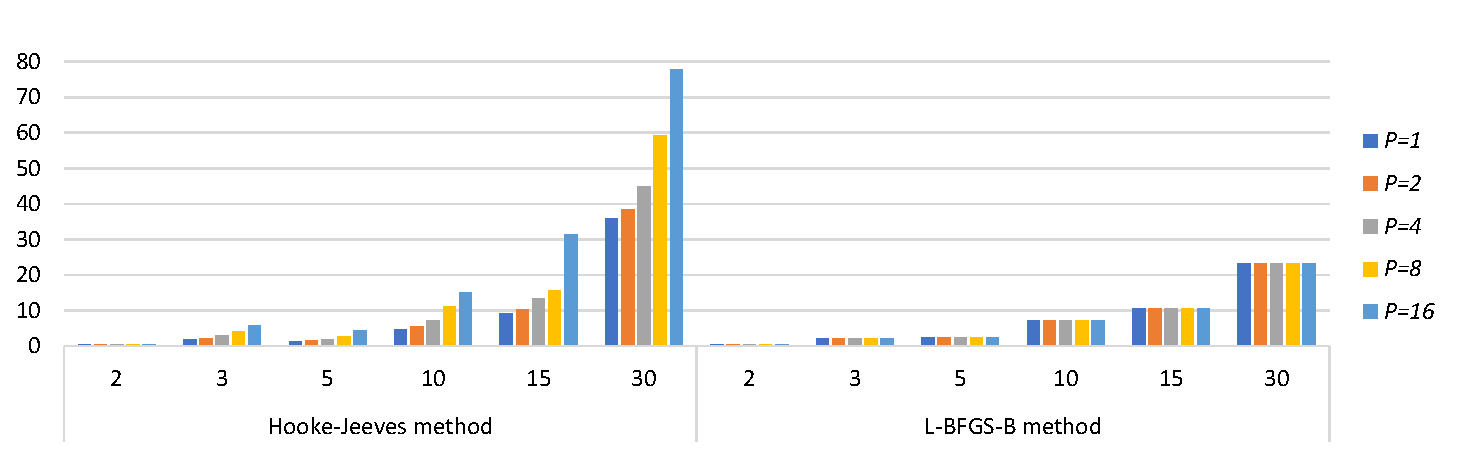
\includegraphics[width=1.0\linewidth]{RosenbrocNT.pdf}
  \caption{Number of trials executed on the Rosenbrock function}
  \label{fig:RosenbrocNT}  
\end{center}
\end{figure}

\begin{figure}
\begin{center}
  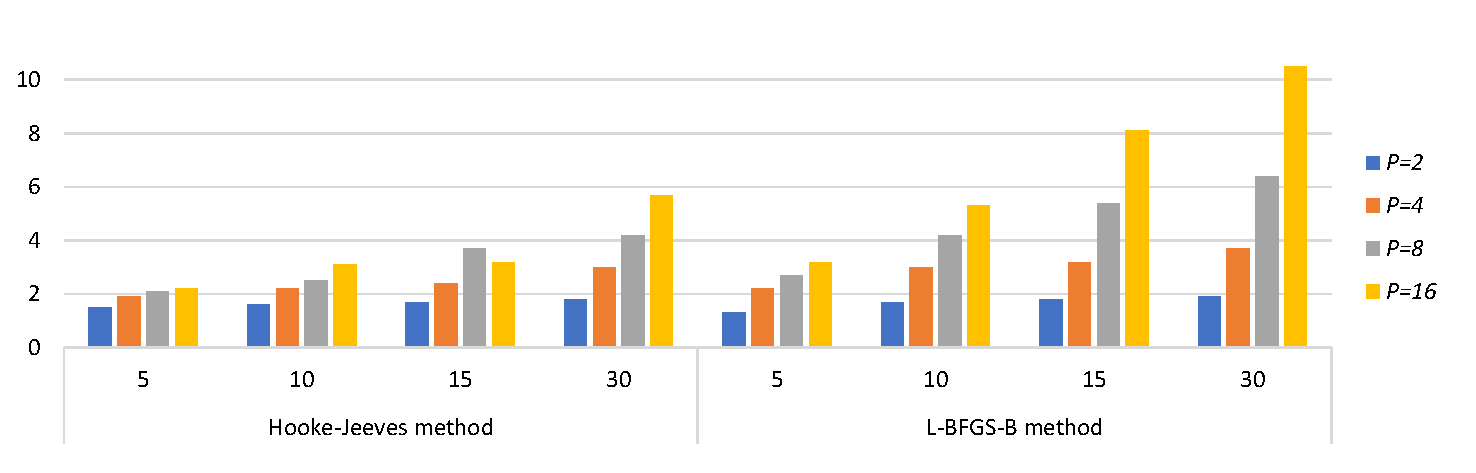
\includegraphics[width=1.0\linewidth]{RosenbrocSpeedup.pdf}
  \caption{Speedup on the Rosenbrock function}
  \label{fig:RosenbrocSpeedup}  
\end{center}
\end{figure}


The results demonstrated the methods of parallelization of the local optimization algorithms described in Section \ref{sec:local} to show good results for the test function. At that, for the problems with low dimensionality (less than 30) Hooke-Jeeves method suited better. However, starting from the dimensionality of 30, L-BFGS-B method begins to execute fewer trials. Also, because of some features of parallelization, Hooke-Jeeves method executes more and more computations of the objective function with in-creasing number of threads, whereas L-BFGS-B always performs the same number of trials. It is explained by the parallelization of the computing of gradient in L-BFGS-B so that the number of computations of the objective function is the same regardless to the number of threads while in Hooke-Jeeves method the algorithm itself is parallelized so that not all the points, at which the trials were executed earlier in the parallel algorithm match the trajectory of the sequential method.

Next, the experiments, which the global search algorithms as well as the local methods have been employed in, were carried out. In \cite{Gaviano2003} GKLS (this abbreviation consists of the first letters of the authors’ names) generator was described. This generator allows generating the multiextremal optimization problems with the properties known \textit{a priori}: the number of local minima, the sizes of the attraction regions of the ones, the global minima points, the objective function value at this point, etc. The test problems generated by this generator are featured by a small time of computing the objective function values.

The global minimum $y^*$ was considered to be found if the algorithm generates a trial point $y^k$ in the $\delta$-nearness of the global minimum, i.e. $\|y^k -y^*\| \leq \delta$. At that, the nearness size was selected (according to \cite{7}) as $\delta = \| b - a \|\sqrt[N]{\Delta}$. Here $N$ is the dimensionality of the problem being solved, $a$ and $b$ are the boundaries of the search domain $D$, the parameter $\Delta = 10^{-6}$ for $N = 4$ and $\Delta = 10^{-7}$ for $N = 5$. When using AGS method, the parameter $r=4.5$ was selected for class Simple, and $r=5.6$ for class Hard; the parameter of the construction of the Peano curve was fixed to be $m=10$. The maximum allowed number of iterations was $K_{max}= 5\cdot10^6$.

The number of iterations for the local methods was limited to $10^4$, the precision of the local methods was set to $10^{-4}$. First, the problems were solved by the global search method with the parameters specified above. Then, a local method was started from the optimal point found to find the minimum more precisely.

Table XX presents the averaged number of iterations, which AGS required to solve the problem. Tables XX and XX present the numbers of trials executed by Hooke-Jeeves and BFGS local methods. Tables XX and XX present the speedups achieved when solving the problem as a whole.

\begin{table}[ht]
	\caption{Averaged number of iterations for AGS algorithm}
	\label{tab:5}
	\center
	\begin{tabular}{|c|c|c|c|c|c|c|}
		\hline
		N & Problem class & P = 1 & P = 2 & P = 4 & P = 8 & P = 16 \\
		\hline 
		    \multirow{2}{*}{4} & hard & 36528 & 18651 & 9854 & 4808 & 2260 \\ \cline{2-7}
		                       & simple & 9995 & 5199 & 2706 & 1333 & 630 \\
		\hline
		    \multirow{2}{*}{5} & hard & 266420 & 149109 & 90894 & 39873 & 22206 \\ \cline{2-7}
		                       & simple & 29853 & 12913 & 7296 & 3618 & 2220 \\
		\hline
	\end{tabular}
\end{table}



%\begin{table}[ht]
%	\caption{Averaged number of trials executed by Hooke-Jeeves method}
%	\label{tab:6}
%	\center
%	\begin{tabular}{|c|c|c|c|c|c|c|}
%		\hline
%		N & Problem class & P = 1 & P = 2 & P = 4 & P = 8 & P = 16 \\
%		\hline 
%		    \multirow{2}{*}{4} & hard &  &  &  &  &  \\ \cline{2-7}
%		                       & simple &  &  &  &  &  \\
%		\hline
%		    \multirow{2}{*}{5} & hard &  &  &  &  &  \\ \cline{2-7}
%		                       & simple &  &  &  &  &  \\
%		\hline
%	\end{tabular}
%\end{table}
%
%\begin{table}[ht]
%	\caption{Speedup when using Hooke-Jeeves method}
%	\label{tab:7}
%	\center
%	\begin{tabular}{|c|c|c|c|c|c|}
%		\hline
%		N & Problem class  & P = 2 & P = 4 & P = 8 & P = 16 \\
%		\hline 
%		    \multirow{2}{*}{4} & hard &  &  &  &  \\ \cline{2-6}
%		                       & simple &  &  &  &  \\
%		\hline
%		    \multirow{2}{*}{5} & hard &  &  &  &  \\ \cline{2-6}
%		                       & simple &  &  &  &  \\
%		\hline
%	\end{tabular}
%\end{table}
%
%
%\begin{table}[ht]
%	\caption{Averaged number of trials executed by BFGS method}
%	\label{tab:8}
%	\center
%	\begin{tabular}{|c|c|c|c|c|c|c|}
%		\hline
%		N & Problem class & P = 1 & P = 2 & P = 4 & P = 8 & P = 16 \\
%		\hline 
%		    \multirow{2}{*}{4} & hard &  &  &  &  &  \\ \cline{2-7}
%		                       & simple &  &  &  &  &  \\
%		\hline
%		    \multirow{2}{*}{5} & hard &  &  &  &  &  \\ \cline{2-7}
%		                       & simple &  &  &  &  &  \\
%		\hline
%	\end{tabular}
%\end{table}
%
%
%\begin{table}[ht]
%	\caption{Speedup when using BFGS method}
%	\label{tab:10}
%	\center
%	\begin{tabular}{|c|c|c|c|c|c|}
%		\hline
%		N & Problem class  & P = 2 & P = 4 & P = 8 & P = 16 \\
%		\hline 
%		    \multirow{2}{*}{4} & hard &  &  &  &  \\ \cline{2-6}
%		                       & simple &  &  &  &  \\
%		\hline
%		    \multirow{2}{*}{5} & hard &  &  &  &  \\ \cline{2-6}
%		                       & simple &  &  &  &  \\
%		\hline
%	\end{tabular}
%\end{table}


\begin{figure}
\begin{center}
  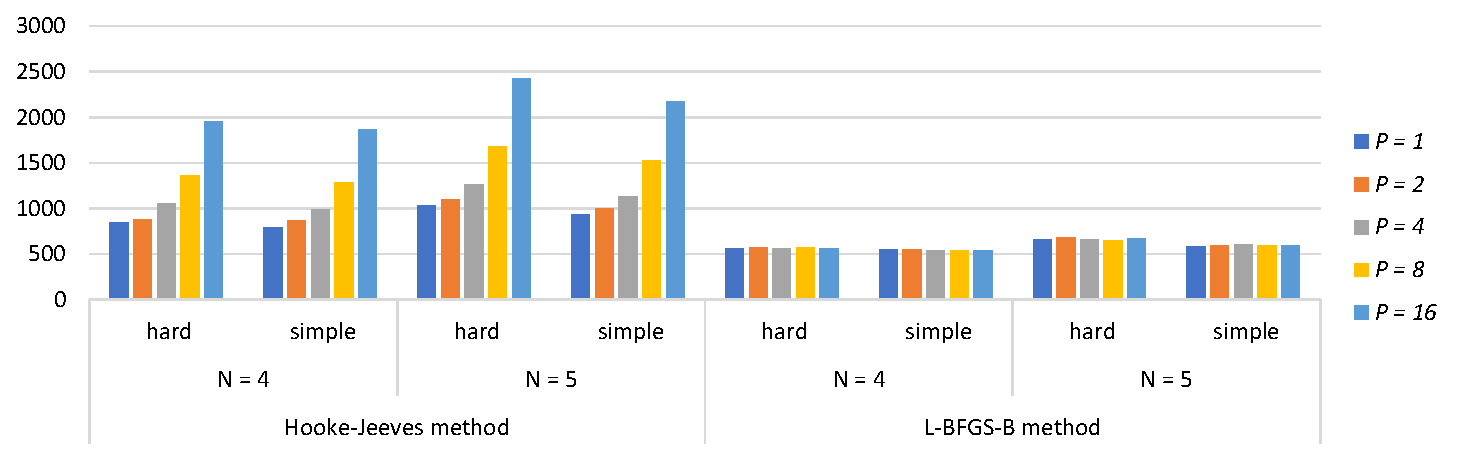
\includegraphics[width=1.0\linewidth]{GKLSNT.pdf}
  \caption{Number of trials executed on the GKLS function}
  \label{fig:GKLSNT}  
\end{center}
\end{figure}

\begin{figure}
\begin{center}
  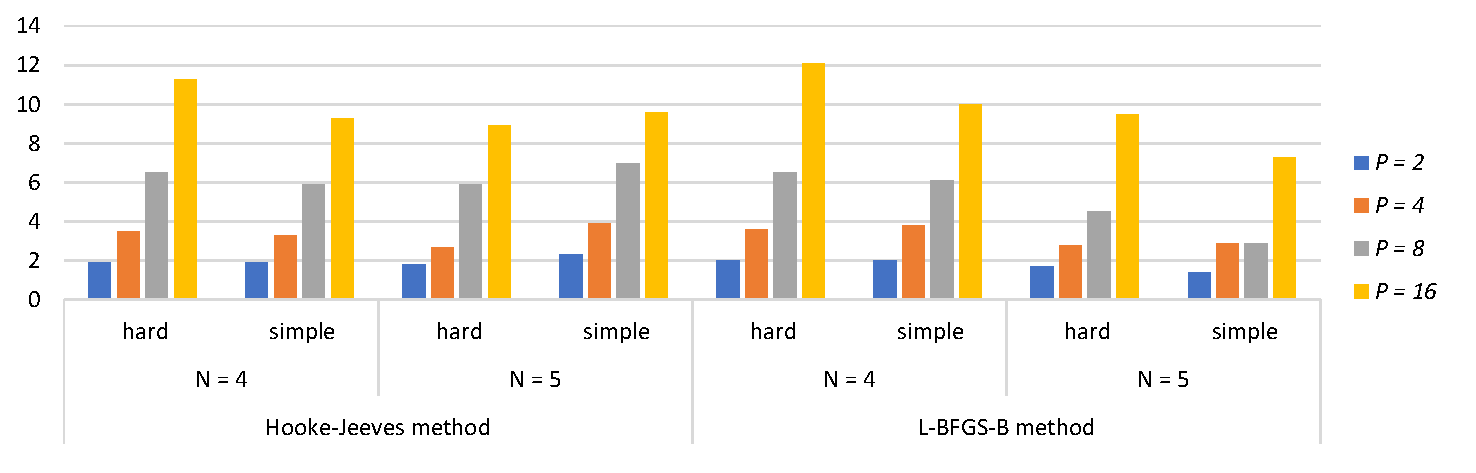
\includegraphics[width=1.0\linewidth]{GKLSSpeedup.pdf}
  \caption{Speedup on the GKLS function}
  \label{fig:GKLSSpeedup}  
\end{center}
\end{figure}


The local methods required less number of trials to refine the solution as compared to the global search method. As a result, the contributions of the local methods into total time of solving the problem were not very large. At that, L-BFGS-B method made much less computations of the objective function.

Within the framework of the last experiment, an applied optimization problem was solved. This problem arose when solving the inverse problem of chemical kinetics.

The reaction investigated and respective experimental data are described in \cite{Uskov2020}. The mathematical model of the chemical kinetics problem comprises a system of differential equations, which describes the variations of the concentrations of substances in time according to the rates of the reaction stages. According to this model, one can formulate an optimization problem, which defines the objective function as a sum of absolute deviations of the calculated concentrations from the ones measured experimentally:
\[
F = \sum_{i=1}^{M} \sum_{j=1}^{N} \mid x_{ij}^{calc} - x_{ij}^{exp}\mid \rightarrow \min,
\]
where $x_{ij}^{calc}$ and $x_{ij}^{exp}$ are the calculated values of concentrations of the components and the ones measured experimentally, respectively; $M$ is the number of measurement points, and $N$ is the number of substances participating in the reaction. The complete problem statement is given in \cite{PAVT}. Here, we note only that the number of the unknown parameters (i.e. the dimensionality of the optimization problem being solved) was 15, and we will consider this one as an optimization problem with a complex ``black-box'' objective function only.

To solve the problem stated, the synchronous parallelization scheme (using MPI) was employed. The number of processes $p$ to compute the function values varied from 1 up to 15. Also, there was an additional managing process, which processed the accumulated search information. In the stopping criteria of the method, the value $\varepsilon=0.01$ was used, the reliability parameter of the method was set as $r = 3$. After the work of GSA, a parallel local method was started to refine the result found, the precision of the local method was set to $10^{-4}$, the limitation on the number of trials was $10^4$. 

Table XX presents the total time of solving four problems corresponding to four different temperature regimes.

%\begin{table}[ht]
%	\caption{Averaged time of solving the problem, sec.}
%	\label{tab:11}
%	\center
%		\begin{tabular}{|c|c|c|c|}
%		\hline
%		%\noalign{\smallskip}
%		Method & P = 1 & P = 3 &  P = 15 \\
%		\hline 
%		Hooke-Jeeves & 2386.4 & 1053.1 & 713.1  \\
%		\hline
%		L-BFGS-B & 2571.7  & 1096.4  & 720.3  \\
%		\hline
%	\end{tabular}
%\end{table}

Table XX presents the data for one of the temperature regimes only (that corresponds to a single optimization problem): the time of solving without the run of a local method (Column GSA), using a sequential local method (Column GSA-l), and using a parallel local method run on 15 processes (GSA-pl).

%\begin{table}[ht]
%	\caption{Time of solving the problem using a local method}
%	\label{tab:12}
%	\center
%		\begin{tabular}{|c|c|c|c|}
%		\hline
%		%\noalign{\smallskip}
%		Method & GSA & GSA-l & GSA-pl \\
%		\hline 
%		Hooke-Jeeves & 158.1 & 299.8  & 177.4 \\
%		\hline
%		L-BFGS-B & 158.1  & 252.5  & 165.6  \\
%		\hline
%	\end{tabular}
%\end{table}

\begin{table}
	\caption{Time of solving the problem}
	\label{tab:last}
	\center
	\begin{tabular}{llllllll}
		\hline\noalign{\smallskip}
		$p$ & \multicolumn{3}{l}{ Total time of solving four problems } & & \multicolumn{3}{l}{One of the temperature regimes only} \\
		\noalign{\smallskip} \cline{2-4} \cline{6-8} \noalign{\smallskip}
		 & P = 1 & P = 3 &  P = 15 & & GSA & GSA-l & GSA-pl  \\
		\noalign{\smallskip} \hline \noalign{\smallskip}
		Hooke-Jeeves & 2386.4 & 1053.1 & 713.1 & & 158.1 & 299.8  & 177.4  \\
		L-BFGS-B & 2571.7  & 1096.4  & 720.3 & & 158.1  & 252.5  & 165.6  \\

		\noalign{\smallskip}\hline
	\end{tabular}
\end{table}

Concluding general results, one can say that the use of local methods at the final stage of search allows solving the optimization problems with higher precision. In many cases, it is enough to use sequential local methods. However, for the problems with complex gully structure of the objective function require parallelizing the whole search process including the local stage as well. In the present work, two local optimization algorithms with the parallelization variants for shared memory as well as for distributed one are described. As the experiments have shown, the methods for parallelizing the local methods (at the final stage of global search) proposed demonstrated good results in solving both the test optimization problems and the applied ones. 

\subsubsection{Acknowledgements} This study was supported by the Russian Science Foundation, project No.\,21-11-00204.

%
% ---- Bibliography ----
%
% BibTeX users should specify bibliography style 'splncs04'.
% References will then be sorted and formatted in the correct style.
%
\bibliographystyle{splncs04}
\bibliography{bibliography}
%
\end{document}
